% GENERATED by assemble_submissions.py -- do not edit.
% Blocks lifted out of the body to hold main content near TMLR's recommended 12 pages; appendices sit after the references and do not count.

\section{The resolution floor of the randomization test}
\label{app:floor}

The argument is worth stating because the floor is a property of the design rather
than of the data. Our statistic is $|\mathrm{mean}(a) - \mathrm{mean}(b)|$. When
the two arms are the same size, the complement of any admissible group-$a$ subset
is itself an admissible group-$a$ subset, and swapping the groups negates the
difference while preserving its absolute value. Every regrouping at the observed
extreme therefore has a partner that is equally extreme, the count can never be
odd at the tail, and the smallest attainable fraction is $2/\binom{n_a+n_b}{n_a}$
rather than $1/\binom{n_a+n_b}{n_a}$. When the arms differ in size the complement
has the wrong size, is not an admissible regrouping, no mirror is forced, and
$1/\binom{n_a+n_b}{n_a}$ becomes attainable.

\section{Multiple-comparison correction}
\label{app:stats}

Correction is Holm--Bonferroni over two \emph{pre-registered} families, declared
before the final arm was trained: Family A (predictive quality, $m=4$, metric
validation task loss) and Family B (adaptive depth, $m=2$, metric depth--difficulty
correlation). The split is declared rather than chosen because the two families ask
different questions on different quantities, and pooling them would correct the
depth claim for tests that cannot bear on it. Holm controls the same familywise
error rate as plain Bonferroni and is uniformly more powerful, and here the choice
is load-bearing: plain Bonferroni over the seven comparisons would give
$0.05/7 = 0.00714$, \emph{below} the floor of 0.00794---a design in which no effect
of any size could be declared significant. Holm's easiest threshold at $m=4$ is
$0.0125$, a margin of 0.0046 above the floor.

Two consequences we hold ourselves to. A declared comparison that could not be run
still consumes its slot: dropping a failed arm must never make the survivors easier
to call significant. And a comparison whose floor exceeds its Holm threshold is
\emph{undecidable} and reported \texttt{N/A}, never ``not significant''---that
phrasing would blame the data for a limit of the design.

\section{Integrity checks and structurally-zero loss terms}
\label{app:integrity}

\subsection{Integrity checks}


Three mechanical invariants hold across the matrix, each enforced by an automated
check rather than by inspection. \textbf{(i) Inputs are bit-identical across arms
for the same record}: feature ranges are identical at $E \in \{1,5,6\}$, so a
difference between arms cannot be a difference in representation. \textbf{(ii) The
regression or classification target is absent from the input}, and no oracle routing
label is encoded into a feature slot. \textbf{(iii) The arms are parameter-matched
to 0.069\%} and the seed-blind configuration is identical within each arm, so
comparability cannot rest on a single code revision: the matrix spans four commits,
and it is the frozen specification plus the config-equality check that holds the
arms comparable, not one revision.

One disclosure belongs with the config table. Three loss terms are structurally
zero on language: the family-classification term because its head reads a detached
representation so its gradient cannot reach the trunk, and the routing-supervision
and halting-supervision terms because natural language supplies no per-token oracle
expert and no per-token oracle depth. The first is a genuine advantage over a
comparable synthetic study, where a family cross-entropy is often one of the larger
terms in the objective and every specialisation claim must be caveated for it.

\section{Loss stratified by token frequency and position}
\label{app:stratified}

\subsection{Stratified loss: the advantage concentrates on hard tokens}
\label{sec:stratified}

Fig.~\ref{fig:stratified} groups validation loss by the frequency decile of the
\emph{target} token---difficulty being a property of what must be predicted, not of
the input---and by position within the block.

Both recursive arms improve most where prediction is hardest. The MoRE$-$MoE
advantage grows from $-0.147$ nats on the most frequent decile to $-0.374$ on the
rarest; MoR's from $-0.188$ to $-0.527$. The widening is not monotone---the gap
dips at the seventh and tenth deciles---so we claim a trend, not a monotone
relationship. Neither architecture's gain is a uniform shift, which is what a
pure capacity effect would look like.

\begin{figure*}[t]
\centering
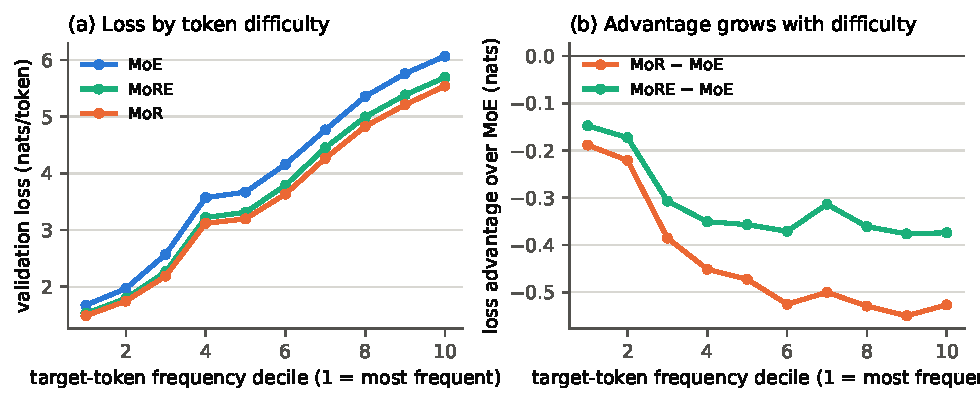
\includegraphics[width=0.98\linewidth]{fig_stratified.pdf}
\caption{(a) Validation loss by target-token frequency decile; decile 1 is the
\emph{most frequent} (easiest) and decile 10 the rarest. (b) Each recursive arm's
advantage over MoE, which widens toward the rarer deciles, though not monotonically.
Exploratory, uncorrected.}
\label{fig:stratified}
\end{figure*}

\textbf{A prediction this does not support.} If recursion were doing what the
adaptive-computation premise suggests---spending steps where context is thin---the
recursive arms should gain most at the \emph{start} of a block. They do the
opposite: MoRE's advantage over MoE is $-0.047$ nats in the first 8 positions and
$-0.359$ in the last 128; MoR's goes from $-0.250$ to $-0.465$. Both recursive arms
gain most where context is \emph{longest}. We report this because it disconfirms a
mechanism we would otherwise have asserted, and because it is consistent with the
capacity account in \S\ref{sec:mechanism}: a shared block iterated is accumulating
representation, not compensating for missing context.

\begin{figure*}[t]
\centering
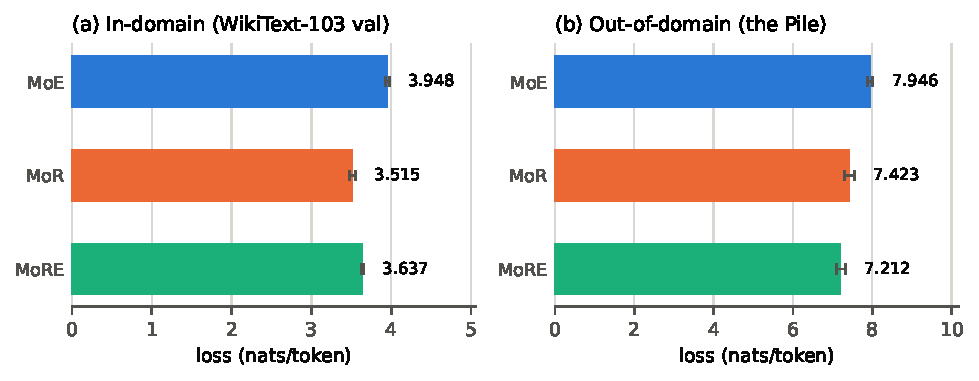
\includegraphics[width=0.98\linewidth]{fig_ood.pdf}
\caption{The ordering inverts out of domain: MoRE is worst in domain (a) and best
on the Pile (b). Same three entities and colours in both panels. Exploratory,
uncorrected.}
\label{fig:ood}
\end{figure*}

\section{The subspace-trapping probes}
\label{app:trapping}

\subsection{A plausible mechanism, refuted}
\label{sec:trapping}

\textbf{[MEASURED; hypothesis falsified.]} The natural explanation for MoRE's
collapse is \emph{subspace trapping}: routing a token once confines its recursion
to a single expert's parameter subspace, and repeated application of one block
within that subspace drives the state toward a fixed point rather than refining it.
It is an appealing account and it is wrong. We tested it three ways.

\begin{center}
\small
\begin{tabular}{lccc}
\toprule
probe & MoE & MoR & MoRE \\
\midrule
participation ratio    & 41.5 & \textbf{70.3} & 57.3 \\
inter-expert cosine    & 0.630 & \textsc{n/a} & 0.916 \\
\bottomrule
\end{tabular}
\end{center}
Participation ratio is the final-state value, $\pm$ 1.6, 5.6 and 2.8 across
seeds respectively; the cosine is the mean between-expert value.

\textbf{(i) Trapping predicts lower participation ratio in the composed arm;
it is higher.} If recursion were collapsing the state onto a low-dimensional
subspace, the composed model's final-state PR should fall below MoE's, since MoE
has no recursion at all. It does not: MoRE's PR is $57.3$ against MoE's $41.5$,
and MoR's---with no routing---is higher still at $70.3$. Recursion \emph{expands}
the effective dimensionality, and routing contracts it somewhat without collapsing
it. The ordering refutes the prediction.

\textbf{(ii) Trapping predicts oscillating or fixed-point dynamics; velocity
decays smoothly.} Measuring the L2 norm of consecutive post-norm states across
depth, both recursive arms decay monotonically---MoR from 11.06 at step 2 to 5.71
at step 7, MoRE from 9.09 to 3.49---which is the signature of settling, not of
vibrating around an attractor.

\textbf{(iii) Trapping predicts that successive updates rescale the state;
they are near-orthogonal.} The mean cosine between a step's update and the state
it updates from is negative in both arms ($-0.26$ to $-0.06$), i.e. updates push
into new directions rather than amplifying existing ones. A rescaling collapse
would show positive collinearity approaching $+1$.

The recursion in this architecture is dynamically healthy: it travels, it settles,
and it adds dimensions. The failure is not a broken iterated map. That rules out
the most attractive explanation and leaves the budget competition
(\S\ref{sec:competition}) as the account the data supports---which is a stronger
position than an unexplained null, because we can say which of the obvious
mechanisms it is \emph{not}.

\section{Matching the parameter budget across the three arms}
\label{app:engine}

\subsection{One engine, three modes}


MoE, MoR and MoRE are configurations of one implementation with an explicit
\texttt{architecture} mode, not three codebases. They share one data pipeline, one
optimiser setup and one evaluation path, so a difference between them cannot be a
difference in the harness. Only the fields their definitions require differ:
$E \in \{6,1,6\}$, $T \in \{1,7,7\}$, MoR's FFN multiplier (below), and the two
loss weights for quantities that do not exist in a given arm (no ponder cost at
depth 1, nothing to balance with one expert).

We write \textbf{MoR} for our recursion-only configuration---one shared block with
adaptive halting---which is in the spirit of weight-tied recursive transformers
with learned halting \citep{dehghani2019ut,bae2025mor} but is not a reproduction
of any specific published system; all three arms are configurations of the same
engine.

\paragraph{Matching the budget.} MoR has one FFN where MoRE has six, so matching
the per-FFN multiplier would compare 5.6M parameters against 0.9M and call the
difference architectural. We instead equalise \emph{total} FFN hidden width,
giving MoR's single FFN a multiplier of $24 = 4 \times 6$. The result is
5{,}584{,}908 parameters for MoE and MoRE, identical, and 5{,}581{,}063 for MoR---a
0.069\% deficit that is six per-expert halt heads, the router and FFN biases. That
residual is irreducible at any integer multiplier, and it runs \emph{against} the
headline result: the arm with slightly fewer parameters is the one that wins in
domain.

\section{Metric definitions}
\label{app:metrics}

\subsection{Metrics}


\textbf{Primary metric: validation task loss}, the final-epoch per-token
cross-entropy in nats. We deliberately do not select on best-epoch validation loss:
that is an order statistic whose downward bias scales with each arm's per-epoch
validation noise, which is not matched across architectures. On all 15 cells
\texttt{best} equals \texttt{last}---the evaluation interval is one epoch and the
curves decrease monotonically---so \emph{no model selection occurred} on either
split. Best-epoch values are reported alongside so the selection effect stays
checkable.

Because the router is unsupervised, expert indices carry no semantic identity, so
raw agreement with any externally defined partition measures label permutation as
much as partition quality. We therefore report AMI \citep{vinh2010ami},
Hungarian-matched accuracy and cluster purity, each against a \emph{per-run
permutation control}: the same metric computed against shuffled linguistic labels,
averaged over 10 draws. The controlled quantity is the z-score of the real value
against that null, not the raw value. The externally defined partition is a
part-of-speech hypothesis about a useful expert split---a hypothesis, not a
functional ground truth---so a router can be better for next-token prediction and
still score low against it. We therefore never call this ``routing accuracy''
without that qualifier.

For depth we report mean steps, exit rates, halt mass, and the Spearman correlation
between per-token depth and per-token difficulty. \textbf{The correlation is only
interpretable when depth has variance to correlate}: on an arm whose tokens almost
all exit at the ceiling, the correlation is computed against a near-constant and a
value near zero is uninformative rather than negative evidence. We report the exit
rates next to every correlation for that reason (\S\ref{sec:halting}).

\section{The subset sweep behind the depth-saturation finding}
\label{app:saturation}

\subsection{Depth saturation is a data-scale effect, not an architectural limit}


\textbf{[MEASURED, four points at fixed hyperparameters.]} MoRE's halting sits at
the ceiling on the full corpus (97.3\% forced-exit, mean depth 6.955 of 7). It is
tempting to read that as the architecture being unable to learn adaptive depth. A
subset sweep falsifies that reading.

\begin{center}
\small
\begin{tabular}{lcc}
\toprule
training data & mean depth & forced exit \\
\midrule
2.5\%             & 2.43 & $\approx 0$ \\
10\%              & 1.92 & $\approx 0$ \\
40\%              & 1.97 & $\approx 0$ \\
100\% (canonical) & 6.96 & 0.973 \\
\bottomrule
\end{tabular}
\end{center}

At every reduced-data point the same model, at the same ponder weight, allocates
depth adaptively---exit rates near zero, mean depth between 1.9 and 2.4, inside a
budget of 7. The collapse appears only at full scale. \textbf{So the failure is a
calibration finding, not an architectural one}: the ponder penalty that produces
adaptive depth on a small corpus cannot hold depth down at this one.

We state the limit of that claim precisely, because the sweep is exploratory
(single seed, subset fraction below 1, and it may never be quoted as a canonical
result). The subset axis is \emph{not} cleanly monotone---2.5\% gives 2.43 but 40\%
gives 1.97---so the honest phrasing is that \emph{saturation emerges somewhere
between 40\% and 100\% of the data}, not that depth is monotone in training steps.
The mechanism is consistent: the ponder term is linear in expected depth, while the
task gradient grows as the model fits, so the fixed penalty is outpaced. Once the
halting sigmoid saturates, its gradient vanishes and the linear-penalty ACT scheme
cannot recover on its own \citep{graves2016act}. \citet{banino2021pondernet}
replaces the linear penalty with a KL divergence against a geometric prior, which
keeps a gradient on the halt head near saturation, and is the principled fix; we
did not run it, and it is named as future work rather than as a result.

\section{Training protocol and hyperparameters}
\label{app:protocol}

\subsection{Training protocol}



Every canonical arm runs at seeds $\{42,43,44,45,46\}$ and is reported as
mean$\,\pm\,$std over five runs. Training is 3 epochs of AdamW (lr $10^{-3}$,
weight decay $10^{-4}$, gradient clipping 1.0, dropout 0.1) with
$d_{\text{model}} = 256$, one block, 4 attention heads, $T = 7$ and batch size 48
on a single laptop GPU. These settings were fixed once, before the comparison, and
not swept per architecture: they are a stable operating point, and no arm was tuned
for itself.

\textbf{Three epochs is a fixed compute budget, not convergence, and we state it
as such.} One epoch is 526{,}320 blocks $\times$ 256 tokens $= 134.7$M tokens
against $\approx$3.4M non-embedding parameters, so the runs sit in an underfitting
regime; the choice of 3 over 2 was made because the halting axis needs more than
two epochs to separate the arms at all, and going to 8 epochs was rejected on cost.
Every arm receives the identical budget, so the comparison is valid even though no
arm is converged. The consequences are stated in \S\ref{sec:limitations}.

\section{BLiMP and EWoK, in full}
\label{app:blimp}

\textbf{Grammatical competence is real but modest, and routing does not buy it.}
On BLiMP \citep{warstadt2020blimp}, 67{,}000 minimal pairs, both recursive arms beat
MoE (58.74\% and 58.36\% against 56.63\%) and MoR is not distinguishable from MoRE
($p = 0.71$). Every arm is above the 50\% floor, so recursion buys measurable
syntactic sensitivity at this scale; adding routing does not add more of it. The
gains concentrate on long-distance agreement phenomena---anaphor agreement and
determiner--noun agreement---which is where a shared iterative block would be
expected to help. We also ran EWoK \citep{ivanova2024ewok}, on which all three arms
sit within noise of the $50\%$ chance floor (49.62, 50.33, 49.95); that is a
statement about the scale of these models, not about the architectures, so we
exclude it from Table~\ref{tab:main} and draw no comparison from it.

\section{Specialisation against per-run controls}
\label{app:specialisation}

The competition has a second face on the canonical corpus, along a different axis.
The routing balance term is load-bearing and cannot be traded away for depth
either: setting it to zero \emph{collapses} the expert load onto a single expert
(load entropy 0.0001) and drives AMI to zero. A near-uniform per-token router
distribution coexisting with balanced load and above-chance specialisation is
therefore not a pathology to be tuned out---and we note that we initially read it
as one before the sweep refuted us (\S\ref{sec:honesty}).

Specialisation itself is real, and measured against per-run controls rather than
against chance. MoRE's AMI is $0.1803 \pm 0.0246$ against a permutation control of
$0.0249$, a controlled z of $13.43$; Hungarian-matched accuracy is $0.3592 \pm
0.0271$ against a control of $0.2464$. MoE's AMI is $0.1637 \pm 0.0478$ against a
control of $0.0364$ ($z = 6.82$), Hungarian $0.3616$ against $0.2966$. Both
six-expert arms find substantial above-chance structure---and, read together, the
two arms are not distinguishable from each other. Routing quality is approximately
the same with recursion as without it, which is the routing half of the
interference result: recursion does not improve routing, and routing does not
preserve adaptive depth, in the same architecture.

